For developing a new sensor is necessary to make a careful simulations. As a tool for simulations TCAD SYNOPSYS was selected. Technology Computer-Aided Design (TCAD) refers to the use of computer simulations to develop and optimize semiconductor processing technologies and devices [1]. There are three tools were used: SPROCESS, SDE and SDEVICE. SPROCESS simulates the fabrication steps in silicon process technologies. SDE is a device editor which builds and edits device structures using geometric operations. SDEVICE simulates the electrical, thermal, and optical characteristics of silicon and compound semiconductor devices [2].

The parameters which should be clarified are the width, depth of implants, distance within/to next layer, position/shift to neighboring layer, the number of layers and optimal doping concentrations for deep implants. As a simulation result, electric field profile for best charge sharing should be obtained. 

The TCAD geometry of the ELAD sensor (fig.2) is contain p-type sensor, 3 layers of n and p deep implants, p-spray isolation, readout implants, readout electrodes, $SiO_2$ and backplane. With the p-spray isolation technique a shallow unstructured p implant provides a doping density that, integrated over depth, exceeds somewhat the oxide surface charge density, thus preventing the buildup of an electron layer below the oxide [3]. The p-spray concentration was chosen according to the value of the breakdown voltage [4]. The shape of implants is described by using an error function. The total sensor thickness is 150 $\mu m$, the pitch size is 55 $\mu m$ in agreement with TimePix3 readout chip. 

\begin{figure}[h]
\center{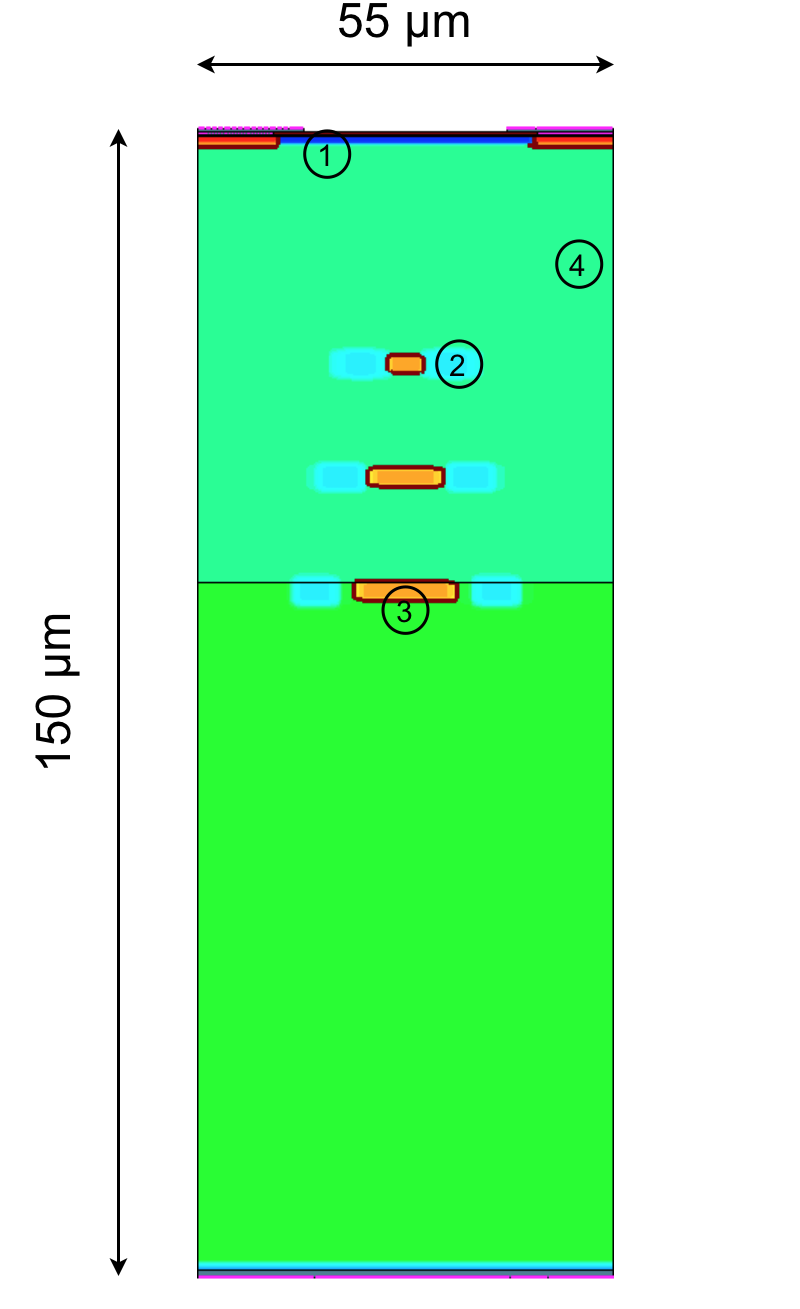
\includegraphics[width=5cm]{/Users/tweety/Documents/PhD/TIPP/TIPP17/pictures/geometry.png}}

Fig. 2. TCAD geometry of the ELAD sensor. 1 - p-spray, 2 - deep p-implant, 3 - deep n-implant, 4 - epi-zone. 
\end{figure}

The TCAD simulation of an electric field shows that the p and n deep implants lead to local changes of potential (fig.3). The mean electric field is similar to an electric field in a standard design sensor, but the local higher dose implants change the field locally, i.e. include an electric field component in $x$ direction. Red zones in fig.3 forces electrons to change their drift path to the right, blue zones to the left, thereby creating the possibility of collecting the charge by two strips. And in addition simulation shows that the non-homogeneous electric field in $x$ direction in the ELAD sensor is stable in time. 

\begin{figure}[h]
\center{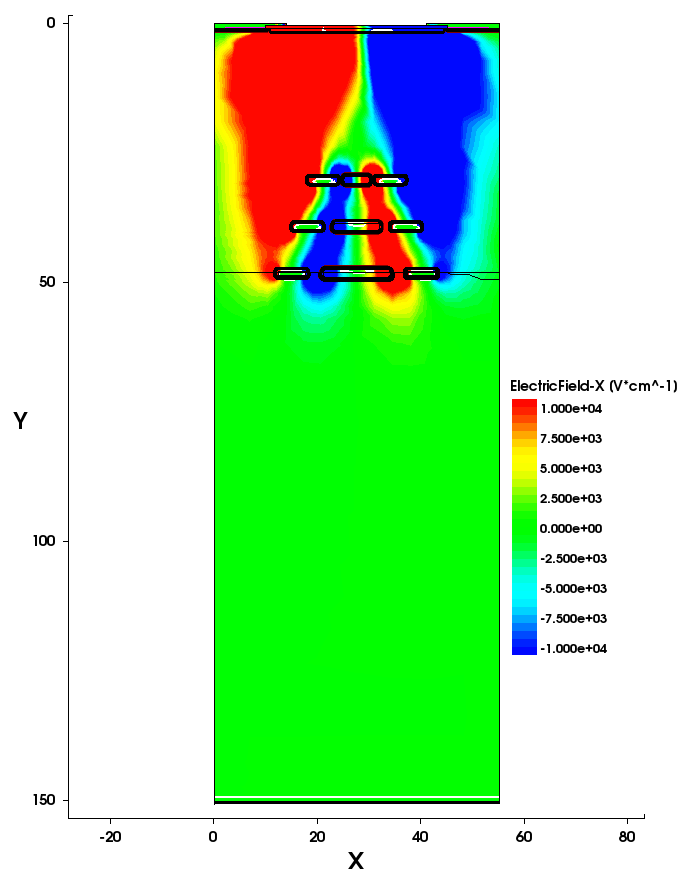
\includegraphics[width=6cm]{/Users/tweety/Documents/PhD/TIPP/TIPP17/pictures/elfield.png}}

Fig. 3. TCAD simulation of the electric field in the ELAD sensor. 
\end{figure}

For understanding the behavior of charge carriers in ELAD sensor the drift simulation was done. The drift simulation shows that the charge carriers created near electrode are collected by it, but the real part of charge i.e. the charge created beneath the deep implants area changes its drift path and collected by two strips (fig.4).  Thereby, the drift simulation proves that the charge sharing in ELAD sensors is possible by using the non-homogeneous electric field in $x$ direction. 


\begin{figure}[h]
\center{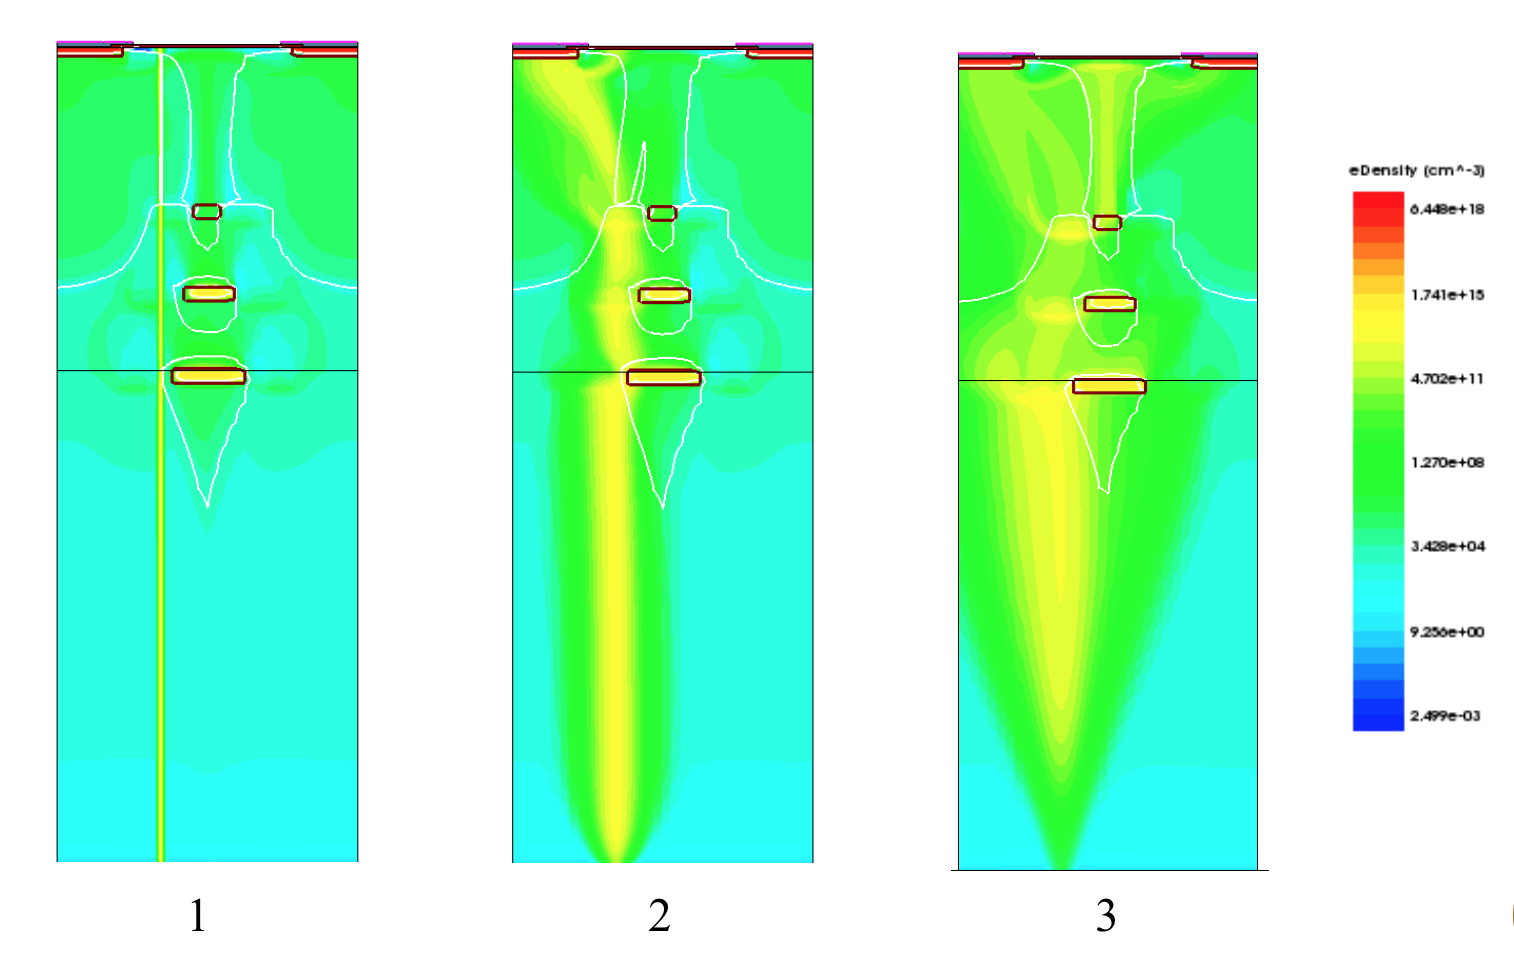
\includegraphics[width=14.2cm]{/Users/tweety/Documents/PhD/TIPP/TIPP17/pictures/drift.png}}

Fig. 4. TCAD drift simulation in the ELAD sensor. 1 - $t = 10^{-12} s$, 2 - $t = 10^{-10} s$, 3 - $t = 1.2 \cdot 10^{-9} s$. 
\end{figure}

